\section{Introduction}
Cable-suspended cooperative transport extends the manipulation capability of small unmanned aerial vehicles beyond the lifting capacity of one aircraft. Transport through infrastructure introduces an additional requirement: the suspended object and the complete supporting formation must change configuration to fit the available space. A lateral opening favors a reduced transverse span, whereas a low ceiling favors a reduced vertical span. An irregular load may also need to rotate substantially to orient a thin dimension toward an opening. Figure~\ref{fig:overview} presents the complete task: a scanned nonconvex payload and its supporting aircraft adopt different configurations while traversing a sequence of spatial restrictions. Here, payload reorientation means a change in its rigid-body attitude, whereas formation reconfiguration means a change in the relative aircraft endpoint positions.

\begin{figure*}[t]
\centering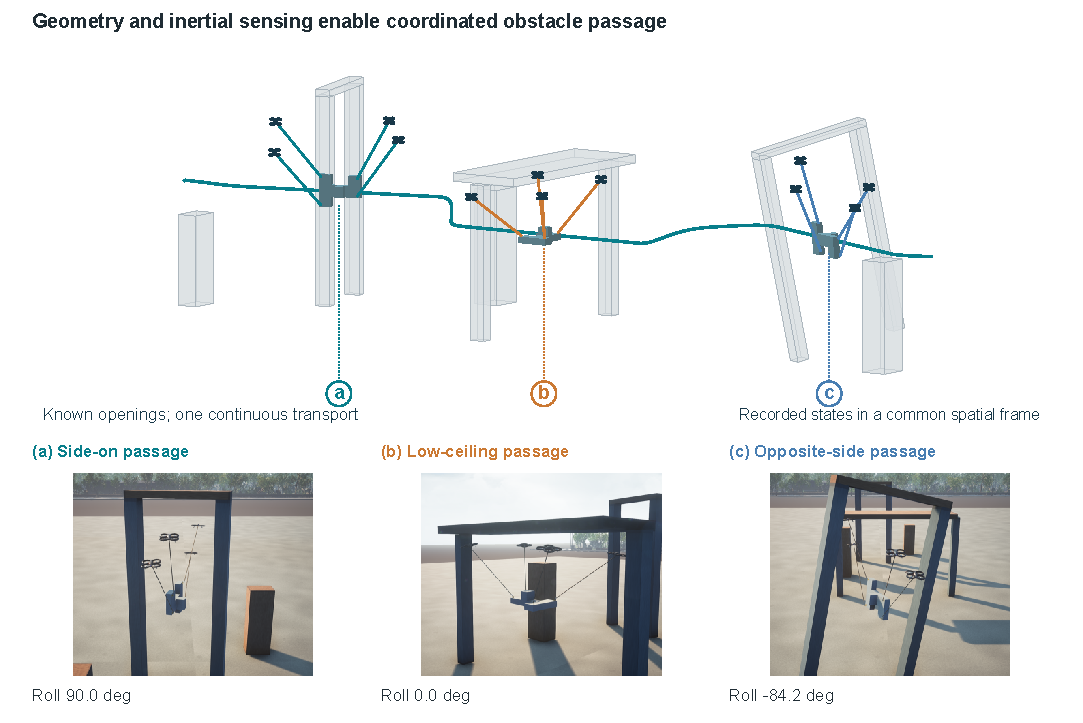
\includegraphics[width=\textwidth]{fig01_overview.pdf}
\caption{Cooperative transport through sequential spatial restrictions. The common-frame spatial view places three recorded payload and support configurations within the known obstacle course. Linked Unreal views show (a) side-on passage through the narrow opening, (b) a spread formation beneath the low ceiling, and (c) opposite-side passage through the tilted opening. Geometry and inertial observations supply the model used for force planning; the load attitude reference family is prescribed. The three configurations belong to one continuous closed-loop simulation.}
\label{fig:overview}
\end{figure*}

Geometry alone cannot determine whether a desired configuration can be sustained. The load center of mass (CoM) generally differs from the centroid of its visible surface, especially when equipment or dense material is distributed unevenly inside the object. A misplaced CoM changes the moment produced by every cable and therefore changes the tension distribution required for a given attitude. Rotational inertia further affects the moments needed during attitude transitions. Because each cable force also determines an aircraft's direction and distance from its attachment, an inertial modeling error changes both tracking behavior and the formation's spatial envelope.

Several strands of research address these issues. Vision and inertial sensing have been used for cooperative cable transport~\cite{li2021}, and nonlinear model predictive control coordinates transportation and load manipulation~\cite{nmpc2023}. Arab et al.~\cite{ast2021} study planning and distributed control for a nonuniform slung load. Load-distribution-based planning~\cite{geng2022} connects the distribution of lifting effort to multilift trajectories. These studies establish that load distribution is a relevant planning variable rather than a consequence to be checked only after a centerline path has been selected.

Agile manipulation also requires the full supporting system to remain feasible. Sun et al.~\cite{sun2025} demonstrate rapid cooperative manipulation using trajectory optimization and incremental nonlinear dynamic inversion. Their evaluations include substantial model mismatch and changing load properties. Thus, agile payload rotation and mismatch-tolerant tracking are established capabilities. Control barrier functions have been used in cooperative manipulation trajectory planning~\cite{pallar2025}, while PolyFly~\cite{polyfly2026} uses polytopic descriptions for collision-free suspended transportation. These approaches motivate evaluating the geometry of aircraft and cables together with that of the payload. Learning-based direct motor control provides another route to cooperative transport~\cite{crazymarl2026}; the present study uses an explicit mechanical model so that estimated moments can be traced through force allocation to formation geometry.

Recent AST studies further clarify the planning context. Chai et al.~\cite{chai2026} investigate time-optimal gap traversal for collaborative aerial transportation with experimental evaluation. Sun et al.~\cite{sunlocal2026} address local obstacle avoidance and trajectory tracking for multi-quadrotor transport. Chan et al.~\cite{chan2026} formulate time-optimal planning of a cable-suspended payload quadcopter using spatial reformulation. The present objective is complementary: given an aperture-conditioned rigid-payload reference family, infer inertial moments from virtual geometry, tension and motion measurements, then propagate them through a compliant force-to-endpoint model. Timing is selected from a finite set; global time optimality and autonomous discovery of the attitude sequence are outside this formulation.

Inertial estimation supplies the complementary information. Petitti et al.~\cite{petitti2020} combine suspended-load inertial estimation with energy-efficient cooperative control. Physically consistent identification relates rigid-body inertial parameters to moments of a nonnegative mass distribution~\cite{wensing2018}. Heins and Schoellig~\cite{heins2025} exploit uncertain inertial parameters and shape information in nonprehensile transportation. These results provide the basis for distinguishing external shape from internal mass properties. A surface scan supports spatial reasoning and constrains possible mass locations; force and motion observations are needed to identify the moments relevant to dynamics.

This paper addresses the connection between measured inertial information and feasible reconfiguration during obstacle passage. We consider a rigid object with calibrated cable attachment points, scanned before transport, and apertures whose geometry is known. The payload translation and attitude are parameterized by smooth, aperture-conditioned references. The planner determines the cable-force history and the resulting compliant endpoint trajectories, together with lowering and timing candidates. The aircraft then track these endpoints through motor and rigid-body dynamics using delayed visual pose feedback. This formulation makes the influence of an identified CoM explicit: it alters the required wrench distribution and, through cable directions, the formation needed to realize the maneuver.

The contribution is an explicit connection from identified inertial moments to constrained support geometry, evaluated under a prescribed payload reference family. First, a sensing-to-configuration formulation combines markerless surface registration, synchronized tension observations and shape-supported integral inertial identification. It provides the mass moments used by the same force and geometry model during transportation. Second, a smooth conic force planner accounts for compliant cable endpoints, aperture halfspaces and aircraft actuation. For near-vertical load attitudes, sequential endpoint separation preserves distinct aircraft positions while the attachment geometry changes orientation. Third, controlled simulations examine three-aircraft and four-aircraft teams, compare identified and uniform-shape models, and demonstrate successive large-angle reorientations of a nonconvex payload through a multi-aperture course. Numerical refinement and an independent continuous command replay examine the underlying mechanical computation.

\begin{figure*}[t]
\centering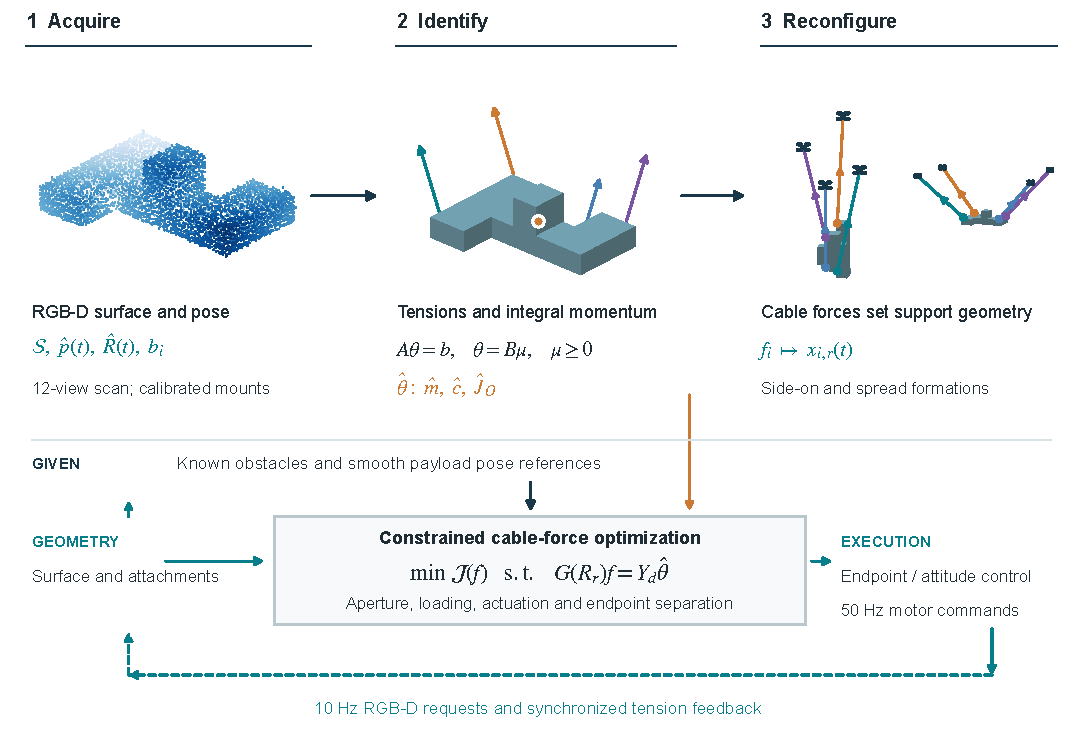
\includegraphics[width=\textwidth]{fig02_framework.pdf}
\caption{Information flow from acquired geometry to supporting formation. Surface and pose registration supplies a common geometric frame; integral momentum and tension observations supply the inertial moments. The known openings and prescribed smooth payload references enter constrained force optimization together with the reconstructed geometry and identified moments. The compliant endpoint map converts cable forces to supporting aircraft positions, followed by motor-driven feedback execution. Point clouds and support configurations use the forked-payload records. The return path denotes visual and tension feedback, rather than online attitude-sequence search.}
\label{fig:framework}
\end{figure*}
